% Практическая работа №3. Цикл for
% Исходный документ: Python _ Практическая работа №3.1 - Цикл for.docx.pdf
% Этот файл — текстовая (LaTeX) копия задания. Сам LMS хранит содержимое
% в базе (src/lms.db, seed в src/db.py), а картинки отдаёт из src/static/.
% Скомпилировать: pdflatex practice3.tex  (или latexmk -pdf practice3.tex)
\documentclass[a4paper,12pt]{article}
\usepackage[T2A]{fontenc}
\usepackage[utf8]{inputenc}
\usepackage[russian]{babel}
\usepackage{amsmath,amssymb}
\usepackage{graphicx}
\usepackage[margin=2.5cm]{geometry}

\graphicspath{{../../static/practice3/}}

\begin{document}

\begin{center}
{\Large\bfseries Практическая работа №3. Цикл for}\\[4pt]
6 заданий $+$ 7-е на дополнительный балл
\end{center}

\medskip
Каждое задание выполняется в отдельном файле. В верхней части файла в комментарии
кратко укажите формулировку выполняемого задания. В остальном коде комментарии не пишутся.

\section*{Задание 1. Задачи с циклом \texttt{for} (9 вариантов)}
Решите свою задачу, используя цикл \texttt{for} (вариант выдаёт преподаватель).
\begin{enumerate}
  \item Двоичное число, введённое пользователем, преобразовать в десятичное число.
  \item Дано число. Найти сумму и произведение его цифр с использованием цикла.
  \item Одноклеточная амёба каждые 3 часа делится на 2 клетки. Определить,
        сколько амёб будет через 3, 6, 9, 12, \dots, 24 часов.
  \item Начав тренировки, спортсмен в первый день пробежал 10 км. Каждый день он
        увеличивал дневную норму на 10\% нормы предыдущего дня. Какой суммарный
        путь пробежит спортсмен за 7 дней?
  \item Дано натуральное число $n$. Среди чисел $1..n$ найти такие, запись которых
        совпадает с последними цифрами записи их квадратов
        (например, $5^2 = 25$, $6^2 = 36$, $25^2 = 625$).
  \item Определить, какие различные цифры входят в заданное целое трёхзначное число.
  \item Определить, из каких цифр состоит заданное трёхзначное число.
  \item Вывести все квадраты натуральных чисел, не превосходящие данного числа $N$.
  \item С клавиатуры последовательно вводится возрастающая последовательность
        10 вещественных чисел и число \texttt{number}. Необходимо определить, между
        какими двумя числами последовательности находится \texttt{number}, и вывести
        их значения и индексы.
\end{enumerate}

\section*{Задание 2. Треугольник из знаков вопроса}
Выведите треугольник $10 \times 10$ из знаков вопроса:
\begin{verbatim}
?
??
???
????
?????
...
??????????
\end{verbatim}

\section*{Задание 3. Треугольник по нечётному $n$}
В зависимости от введённого нечётного значения $n$ выведите треугольник:
\begin{verbatim}
n = 3    n = 5     n = 7
?        ?         ?
??       ??        ??
?        ???       ???
         ??        ????
         ?         ???
                   ??
                   ?
\end{verbatim}

\section*{Задание 4. Сумма факториалов}
Напишите программу, которая вычисляет сумму факториалов всех чисел от 1 до $n$.
Например, для $n = 4$:
\[ 1! + 2! + 3! + 4! = 1 + 2 + 6 + 24 = 33. \]

\section*{Задание 5. Пилообразная последовательность}
Проверьте, является ли последовательность чисел «пилообразной» — каждый элемент
либо больше обоих соседей, либо меньше обоих соседей.

\section*{Задание 6. Числа от 1 до 20 и обратно}
Выведите при помощи одного цикла числа от 1 до 20 и от 20 до 1, где элементы идут
сначала в порядке возрастания, потом убывания.

\section*{Задание 7 (доп. балл). Таблица значений $y(x)$}
Выведите на экран таблицу значений функции $y(x)$ для $x$, изменяющегося
от $a = 0{,}1$ до $b = 1{,}2$ с шагом $h = 0{,}1$. Для решения задачи используйте
цикл \texttt{for}. Вариант функции выдаёт преподаватель.

\medskip
Варианты функций $y(x)$ (нумерованные карточки на картинке ниже):
\begin{center}
  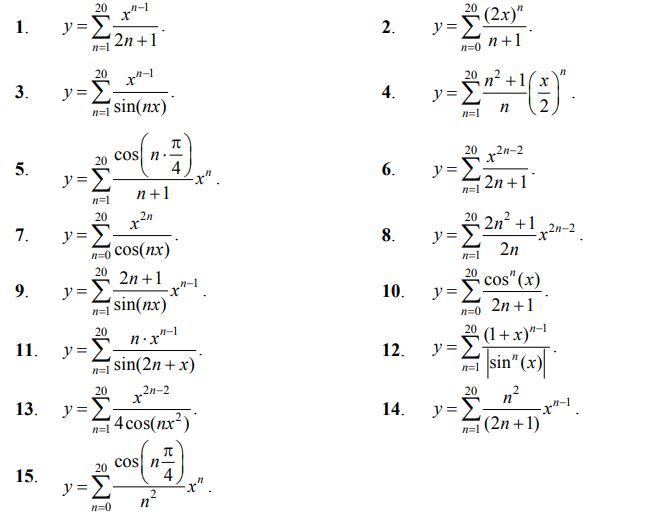
\includegraphics[width=\linewidth]{formulas.png}
\end{center}

\end{document}
